% #############################################################################
% This is Chapter 6
% !TEX root = ../main.tex
% #############################################################################
% Change the Name of the Chapter i the following line
\fancychapter{Results \& Evaluation}
\cleardoublepage
% The following line allows to ref this chapter
\label{chap:results}

So far we have introduced the theme to be developed in this thesis \ref{chap:intro}, we have presented some studies developed in this area \ref{chap:background}, we have presented the concrete case studied in this thesis and we propose a schematization of the work to be developed \ref{chap:architecture}, we have introduced the models that we will implement \ref{chap:Model}, and we have described in detail both the datasets used, as well as the experimental process implemented in this study \ref{chap:implementation}. In this chapter, we present the results obtained in this thesis as well as a discussion section.


\section{Algorithm selection} \label{chap5:framework}

In this section, the process of training and validation of the 8 proposed architectures begins. In a first stage the architectures are trained and validated in order to regulate the hyperparameters of each layer. It is in this stage that the performance of each architecture is also evaluated for the training and validation scenario. In a second stage, XXXX


\subsection{Stage 1 - Hyperparameter tuning}\label{sec:part1}
Beginning with stage 1, in the first part of the process, the focus was to optimize the hypterparameters of the eight proposed architectures. The datasets 1, 2 and 3 represented in Figure \ref{hyptun} were then used, each one consisting of a total of 5 weeks of data, 4 of which were used for training and 1 for validation. Each of the eight architectures went through this process for each of the 3 datasets.  

\begin{figure}[h!]
    \centering
    \begin{center}
    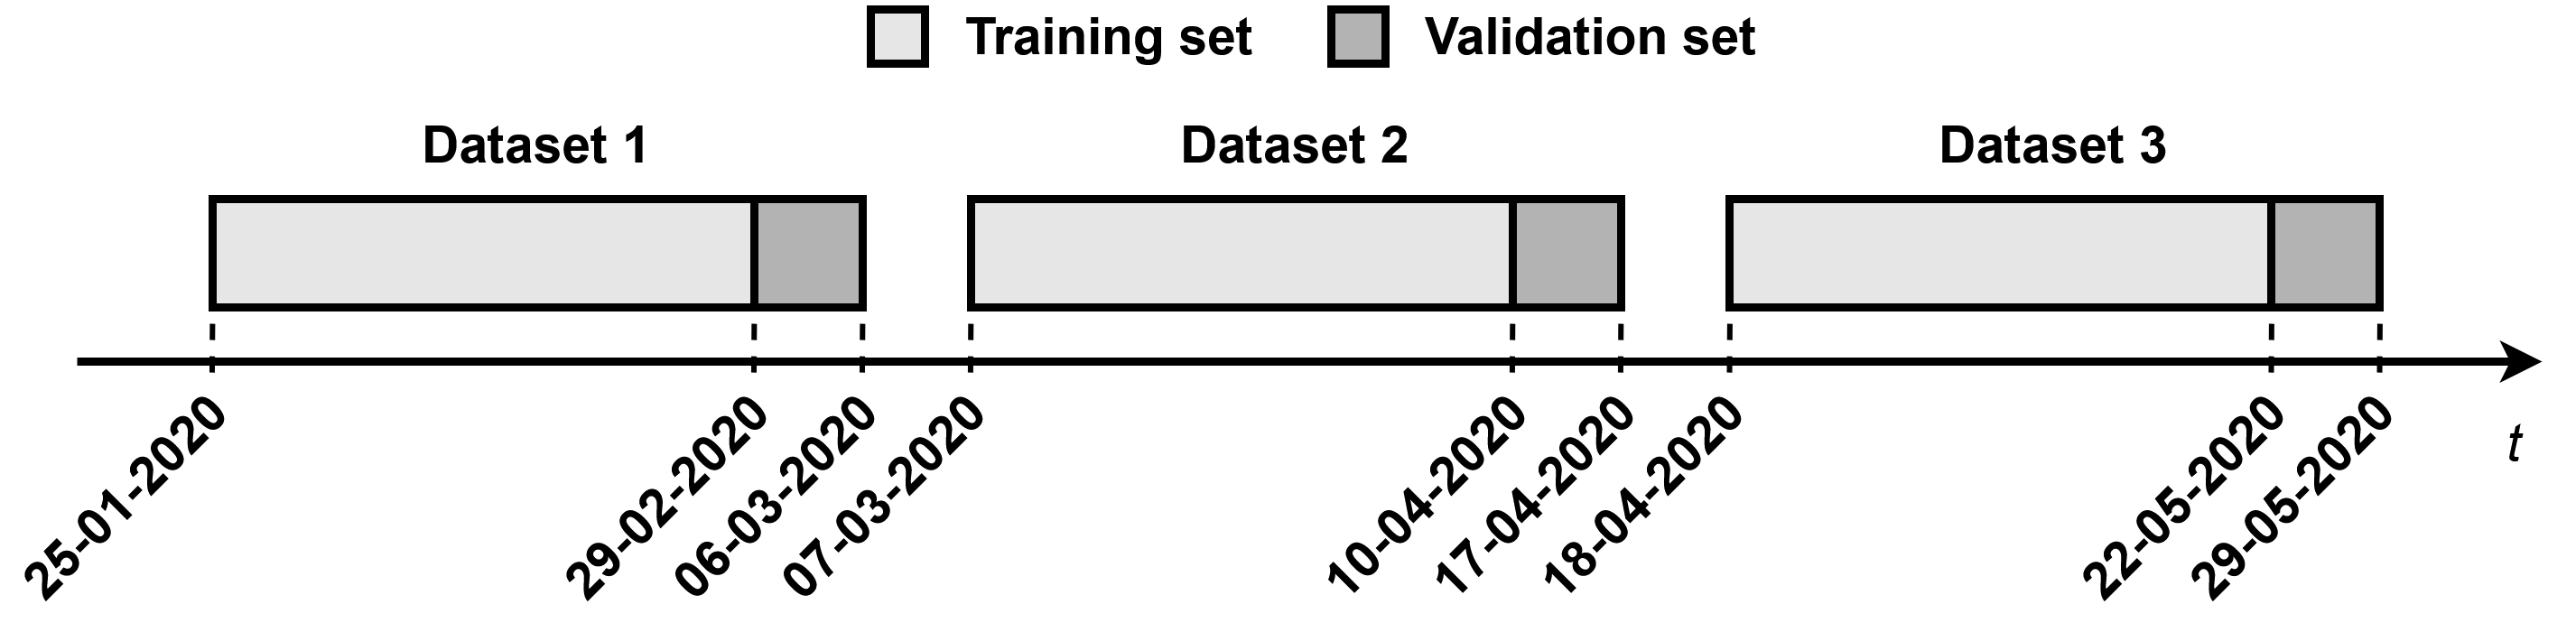
\includegraphics[width=1\textwidth]{Images/hyptun.png}
    \caption{Datasets used for training and validation.}
    \label{hyptun}
    \end{center}
\end{figure}

Models 0 and 1 only consist of a \ac{GRU} or a \ac{LSTM} layer. In this type of layers, the hyperparameter that can be changed is the number of Units - A positive integer that represents the dimensionality of the output space. In models 4, 5, 6 and 7, since they have two distinct layers, the same parameter can be tuned for each one of the layers. In models 2 and 3, the parameters that can change are the number of filters of the \ac{1D CNN} - An integer that represents dimensionality of the output space (i.e. the number of output filters in the convolution), the kernel\_size of the \ac{1D CNN} - An integer or tuple/list of a single integer, specifying the length of the 1D convolution window used, and again, and the number of Units of the \ac{GRU} or \ac{LSTM} layer. 


Since the process of tuning the hyperparameters is done by hand, all the architectures started this phase with layers of 8 units. In models 2 and 3 the initial number of filters of the \ac{1D CNN} layers was also 8 and the kernel\_size used was 10. If the models behaved well in the validation set and showed no signs of overfitting or underfitting, the initial values would be maintained. If signs of overfitting 



If any of these behaviors were observed in at least one of the datasets, the hyperparameters would be changed until the model presented the desired behavior for all the datasets. It was chosen to start with simple architectures and one would only increase the complexity of the architecture (increasing the number of units per layer, for example) if the model did not present all the desired behavior. The increase in the complexity of the model is associated with an increase in its training time, so it was essential to use models as simple as possible. In table \ref{table4}, one can then observe the results of the errors calculated in this process for each of the eight architectures, in each of the three datasets, in the training and validation process.

% Table generated by Excel2LaTeX from sheet 'Sheet6'
\begin{table}[htbp]
  \centering
  \caption{Add caption}
    \begin{tabular}{r|cccccccc}
    \toprule
    \multicolumn{1}{c|}{\textbf{Model}} & 0     & 1     & 2     & 3     & 4     & 5     & 6     & 7 \\
    \midrule
    \# inputs & 15    & 15    & 15    & 15    & 15    & 15    & 15    & 15 \\
    \# hidden layers & 1     & 2     & 3     & 4     & 4     & 4     & 4     & 4 \\
    \# hidden nodes & 8     & 16    & 16    & 16    & 16    & 16    & 16    & 16 \\
    \# outputs & 3     & 3     & 3     & 3     & 3     & 3     & 3     & 3 \\
    \midrule
    \multicolumn{1}{c|}{\textbf{Model}} & \multicolumn{2}{c}{0} & \multicolumn{2}{c}{1} & \multicolumn{2}{c}{2} & \multicolumn{2}{c}{3} \\
    \midrule
    Layout & \multicolumn{2}{c}{Input (15)} & \multicolumn{2}{c}{Input (15)} & \multicolumn{2}{c}{Input (15)} & \multicolumn{2}{c}{Input (15)} \\
          & \multicolumn{2}{c}{GRU (8)} & \multicolumn{2}{c}{LSTM (8)} & \multicolumn{2}{c}{Conv1D (8, 10)} & \multicolumn{2}{c}{Conv1D (8,10)} \\
          & \multicolumn{2}{c}{Dense (3)} & \multicolumn{2}{c}{Dropout (0.2)} & \multicolumn{2}{c}{Maxpooling(10)} & \multicolumn{2}{c}{Maxpooling(10)} \\
          & \multicolumn{2}{c}{} & \multicolumn{2}{c}{Dense (3)} & \multicolumn{2}{c}{GRU (8)} & \multicolumn{2}{c}{LSTM (8)} \\
          & \multicolumn{2}{c}{} & \multicolumn{2}{c}{} & \multicolumn{2}{c}{Dense (3)} & \multicolumn{2}{c}{Dropout (0.2)} \\
          & \multicolumn{2}{c}{} & \multicolumn{2}{c}{} & \multicolumn{2}{c}{} & \multicolumn{2}{c}{Dense (3)} \\
    \midrule
    \multicolumn{1}{c|}{\textbf{Model}} & \multicolumn{2}{c}{4} & \multicolumn{2}{c}{5} & \multicolumn{2}{c}{6} & \multicolumn{2}{c}{7} \\
    \midrule
    Layout & \multicolumn{2}{c}{Input (15)} & \multicolumn{2}{c}{Input (15)} & \multicolumn{2}{c}{Input (15)} & \multicolumn{2}{c}{Input (15)} \\
          & \multicolumn{2}{c}{GRU (8)} & \multicolumn{2}{c}{LSTM (8)} & \multicolumn{2}{c}{GRU (8)} & \multicolumn{2}{c}{LSTM (8)} \\
          & \multicolumn{2}{c}{Dropout (0.2)} & \multicolumn{2}{c}{Dropout (0.2)} & \multicolumn{2}{c}{Dropout (0.2)} & \multicolumn{2}{c}{Dropout (0.2)} \\
          & \multicolumn{2}{c}{GRU (8)} & \multicolumn{2}{c}{LSTM (8)} & \multicolumn{2}{c}{LSTM (8)} & \multicolumn{2}{c}{GRU (8)} \\
          & \multicolumn{2}{c}{Dropout (0.2)} & \multicolumn{2}{c}{Dropout (0.2)} & \multicolumn{2}{c}{Dropout (0.2)} & \multicolumn{2}{c}{Dropout (0.2)} \\
          & \multicolumn{2}{c}{Dense (3)} & \multicolumn{2}{c}{Dense (3)} & \multicolumn{2}{c}{Dense (3)} & \multicolumn{2}{c}{Dense (3)} \\
    \end{tabular}%
  \label{tab:addlabel}%
\end{table}%









% Table generated by Excel2LaTeX from sheet 'Tables Total'
\begin{table}[htbp]
  \centering
  \caption{Stage 1 - Block cross-validation results.}
    \begin{tabular}{cr|cccccccc}
    \toprule
    \multicolumn{1}{l}{\textbf{Model}} &       & 0     & 1     & 2     & \textbf{3} & 4     & 5     & 6     & 7 \\
    \midrule
    \multicolumn{2}{l|}{\textbf{Training Score (t+5)}} &       &       &       &       &       &       &       &  \\
          & RMSE (E+03) & 29.49 & 27.62 & \textbf{26.24} & \textbf{26.43} & 28.00 & 30.12 & 29.23 & \textbf{27.55} \\
          & MAE (E+03) & 22.25 & \textbf{20.42} & \textbf{19.84} & \textbf{19.62} & 20.65 & 22.34 & 21.57 & 20.46 \\
    \multicolumn{2}{l|}{\textbf{Training Score (t+10)}} &       &       &       &       &       &       &       &  \\
          & RMSE (E+03) & 34.13 & 32.81 & \textbf{32.13} & \textbf{32.05} & 32.92 & 34.19 & 34.17 & \textbf{32.31} \\
          & MAE (E+03) & 25.65 & 24.28 & \textbf{24.11} & \textbf{23.77} & 24.34 & 25.32 & 25.30 & \textbf{23.97} \\
    \multicolumn{2}{l|}{\textbf{Training Score (t+15)}} &       &       &       &       &       &       &       &  \\
          & RMSE (E+03) & 37.26 & \textbf{36.19} & 36.23 & \textbf{36.13} & 36.38 & 37.45 & 37.31 & \textbf{35.69} \\
          & MAE (E+03) & 27.93 & \textbf{26.80} & 27.20 & 26.95 & \textbf{26.94} & 27.81 & 27.61 & \textbf{26.48} \\
    \midrule
    \multicolumn{2}{l|}{\textbf{Validation Score (t+5)}} &       &       &       &       &       &       &       &  \\
          & RMSE (E+03) & 39.97 & 33.59 & \textbf{29.11} & \textbf{26.96} & \textbf{30.86} & 35.05 & 39.21 & 35.99 \\
          & MAE (E+03) & 30.06 & 25.58 & \textbf{21.14} & \textbf{20.58} & \textbf{23.97} & 26.77 & 28.96 & 27.90 \\
    \multicolumn{2}{l|}{\textbf{Validation Score (t+10)}} &       &       &       &       &       &       &       &  \\
          & RMSE (E+03) & 46.67 & 35.62 & \textbf{35.59} & \textbf{32.21} & \textbf{34.64} & 37.93 & 41.82 & 39.05 \\
          & MAE (E+03) & 34.80 & 27.59 & \textbf{26.38} & \textbf{24.69} & \textbf{26.92} & 28.89 & 31.54 & 30.26 \\
    \multicolumn{2}{l|}{\textbf{Validation Score (t+15)}} &       &       &       &       &       &       &       &  \\
          & RMSE (E+03) & 48.04 & \textbf{37.87} & 38.11 & \textbf{36.45} & \textbf{37.30} & 41.10 & 43.03 & 41.59 \\
          & MAE (E+03) & 36.29 & 29.35 & \textbf{28.68} & \textbf{28.08} & \textbf{28.81} & 31.47 & 32.40 & 32.13 \\
    \end{tabular}%
  \label{tab:addlabel}%
\end{table}%







By examining the results of the xxx table, 

The three best models are then....xxxxxxxxxxx





\subsection{Stage 2 - Situational study}

In the second stage of the process, the main objective is to compare the 3 models chosen in Stage 1, situationally. To bring this into practice, multiple subdasets were created presenting thre particular situations in the activity of the building: weekdays, weekends and national holidays.

This step serves to identify which model presents the best performance depending on the situation to be expected. If it is possible to define a model that is clearly better to predict certain situations, and another that presents better performance in others, there is the possibility of creating a superior abstraction layer capable of choosing the best model to use in a given scenario. 





For each of the cases presented, XXX dataset was created whose validation subset represents the scenario to be tested. In order to understand which of the 3 models presents the best performance for each scenario, the equation \ref{err_av} was used again. Applying a specific case, the best model to apply in a holiday scenario will be the one that presents on average the lowest error value in the XX scenarios where it was tested.

\subsection{Stage 3 - Model performance}

\begin{figure}[h!]
    \centering
    \begin{center}
    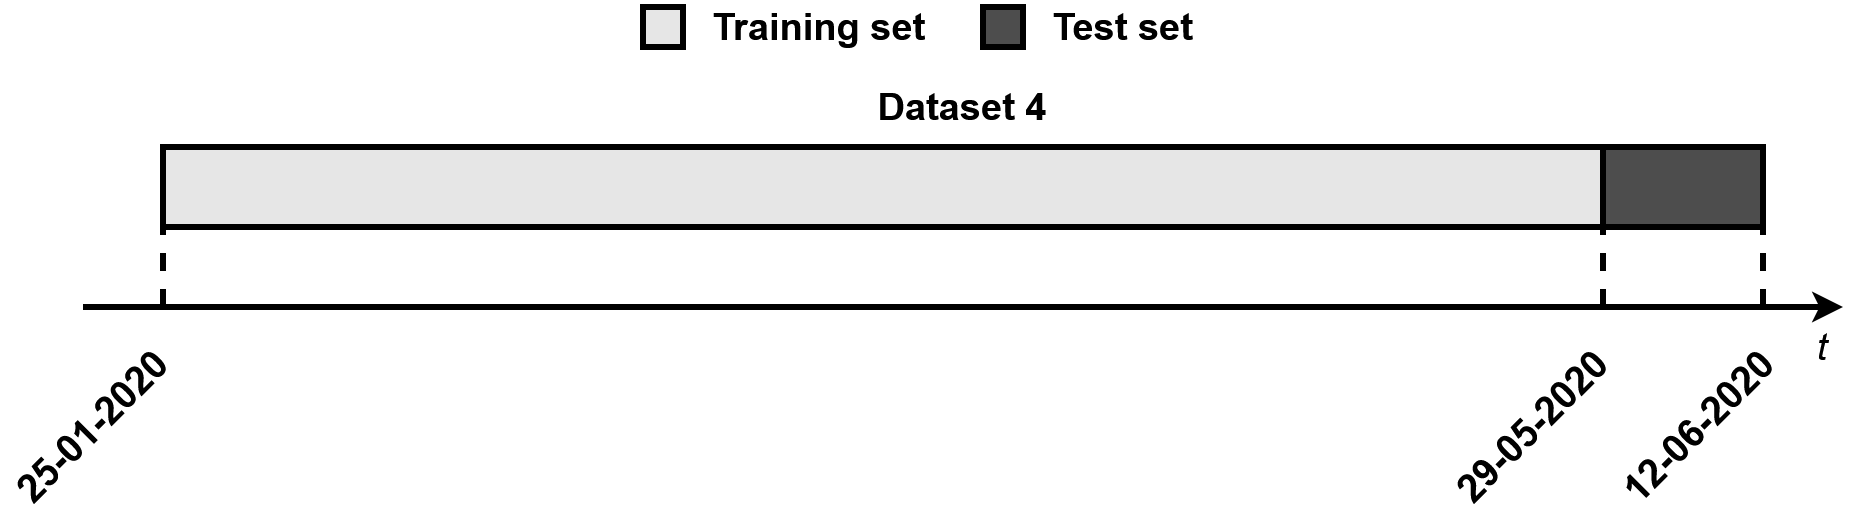
\includegraphics[width=1\textwidth]{Images/Test.png}
    \caption{Dataset used for testing.}
    \label{test}
    \end{center}
\end{figure}


\subsection{Stage 4 - Final system}
\subsubsection{Comparative analysis}

\section{Discussion}

